\documentclass[12pt, letterpaper]{../assignment}
\usepackage{graphicx}
\usepackage{courier}
\usepackage{minted}
\usepackage{amsmath}
\usepackage{polynom}
\usepackage{commath}
\usepackage{amssymb}
\usepackage{amsfonts} 
\usepackage{color}
\usepackage{cancel}
\usepackage{enumitem}
\usepackage{graphicx}
\usepackage{multirow}
\usepackage{float}
\usepackage{bm}
\usepackage{tikz}
\usetikzlibrary{shapes,arrows}
\usepackage{booktabs}
\usetikzlibrary{patterns}

% Define Theme Colors
\definecolor{light-gray}{rgb}{0.2,0.2,0.2}
\definecolor{header-blue}{rgb}{0,0,0.7}
% \definecolor{header-blue}{rgb}{0.5137,0.8353,0.9176}
\definecolor{header-blue}{rgb}{0,0.8,0.95}
\definecolor{dark-gray}{rgb}{0.1,0.1,0.1}
\pagecolor{dark-gray}
\color{white}

\usemintedstyle{monokai}
\oddsidemargin = 0pt
\exercisesheet{Module 5}{Assignment}
\student{Austin Barrilleaux}
\university{\color{header-blue}Johns Hopkins University}
\school{\color{header-blue}Whiting School of Engineering}
\courselabel{EN 535.612}
\semester{Fall 2024}
\usepackage[backend=bibtex,style=numeric,sorting=none]{biblatex}
\bibliography{reference}

\definecolor{light-gray}{rgb}{0.2,0.2,0.2}
\setminted{bgcolor=light-gray,frame=lines,rulecolor=white}
\setlength{\parindent}{0pt}

\makeatletter
\patchcmd{\minted@colorbg}{\noindent}{\medskip\noindent}{}{}
\apptocmd{\endminted@colorbg}{\par\medskip}{}{}
\makeatother

\begin{document}

\subsection*{Problem 1: EXERCISE 5.13}
\subsubsection*{The $\bm{x}$ axis forms a diagonal intersecting the centroid of the homogeneous cylinder.
Determine the inertia properties of the cylinder with respect to $\bm{xyz}$.}

\begin{figure}[H]
    \centering
    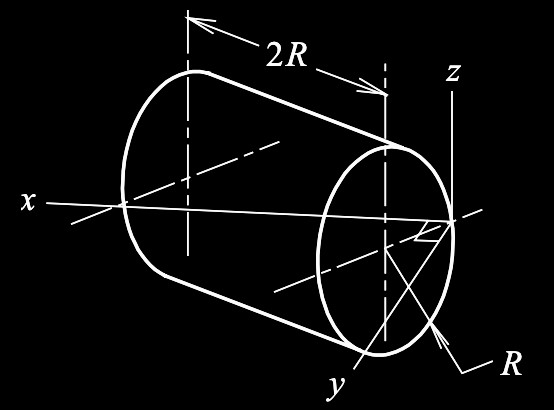
\includegraphics[scale=0.7,frame]{images/Q5_13.png}
\end{figure}

For this problem,
we will define the body frame of the cylinder as:


\begin{center}
\tikzset{every picture/.style={line width=0.75pt}} %set default line width to 0.75pt        

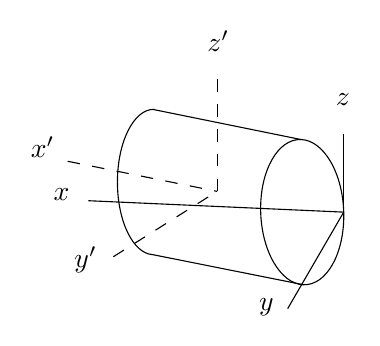
\begin{tikzpicture}[x=0.75pt,y=0.75pt,yscale=-1,xscale=1]
%uncomment if require: \path (0,235); %set diagram left start at 0, and has height of 235

%Shape: Ellipse [id:dp548769057305911] 
\draw   (178.63,157.99) .. controls (167.57,157.62) and (158.33,141.65) .. (157.98,122.33) .. controls (157.64,103) and (166.32,87.63) .. (177.37,88.01) .. controls (188.43,88.38) and (197.67,104.35) .. (198.02,123.67) .. controls (198.36,143) and (189.68,158.37) .. (178.63,157.99) -- cycle ;
%Straight Lines [id:da1570272230512686] 
\draw    (106,73.5) -- (177.36,88.01) ;
%Straight Lines [id:da9673755868087144] 
\draw    (106.02,143.49) -- (178.63,157.99) ;
%Shape: Arc [id:dp9126003894708585] 
\draw  [draw opacity=0] (106.02,143.49) .. controls (96.57,143) and (88.98,127.51) .. (88.98,108.49) .. controls (88.98,89.15) and (96.82,73.48) .. (106.49,73.48) .. controls (106.62,73.48) and (106.75,73.48) .. (106.89,73.49) -- (106.49,108.49) -- cycle ; \draw   (106.02,143.49) .. controls (96.57,143) and (88.98,127.51) .. (88.98,108.49) .. controls (88.98,89.15) and (96.82,73.48) .. (106.49,73.48) .. controls (106.62,73.48) and (106.75,73.48) .. (106.89,73.49) ;  
%Straight Lines [id:da5808049361775272] 
\draw  [dash pattern={on 4.5pt off 4.5pt}]  (137,113) -- (137,58.5) ;
%Straight Lines [id:da4666736331918626] 
\draw  [dash pattern={on 4.5pt off 4.5pt}]  (65,98.5) -- (137,113) ;
%Straight Lines [id:da42223753773815553] 
\draw  [dash pattern={on 4.5pt off 4.5pt}]  (87,144.5) -- (137,113) ;
%Straight Lines [id:da0341392110595069] 
\draw    (198,123) -- (198,85.5) ;
%Straight Lines [id:da8816042449400916] 
\draw    (75,117.5) -- (198,123) ;
%Straight Lines [id:da35220154521105873] 
\draw    (171,169.5) -- (198,123) ;

% Text Node
\draw (46,85.4) node [anchor=north west][inner sep=0.75pt]    {$x'$};
% Text Node
\draw (131,34.4) node [anchor=north west][inner sep=0.75pt]    {$z'$};
% Text Node
\draw (67,138.4) node [anchor=north west][inner sep=0.75pt]    {$y'$};
% Text Node
\draw (57,110.4) node [anchor=north west][inner sep=0.75pt]    {$x$};
% Text Node
\draw (193,64.4) node [anchor=north west][inner sep=0.75pt]    {$z$};
% Text Node
\draw (156,163.4) node [anchor=north west][inner sep=0.75pt]    {$y$};

\end{tikzpicture}
\end{center}

From textbook Appendix,
the centroidal inertia mass properties of a homogeneous cylinder where in the body frame as I defined it are:

\begin{equation*}
    \begin{aligned}
        I_{xx} &= \frac{1}{2} m R^2 & \\
        I_{yy} &= \frac{1}{12} m \left(3 R^2+h^2\right) &= \frac{7}{12} m R^2\\
        I_{zz} &= \frac{1}{12} m \left(3 R^2+h^2\right) &= \frac{7}{12} m R^2\\
    \end{aligned}
\end{equation*}

This expressed the inertia tensor is:

$$ I_{x'y'z'} = \left[\begin{array}{ccc} \frac{1}{2} m R^2 & 0 & 0\\
    0 & \frac{7}{12} m\,R^2 & 0\\ 0 & 0 & \frac{7}{12}m\,R^2 \end{array}\right] $$

The distance from the body frame is:

$$ d = \left[\begin{array}{c} R\\ R\\ 0 \end{array}\right] $$

Using the parallel axis theorem to get the parallel axis transformation of inertia matrix
relative to the center of the frame of reference in question:

$$ I_{pat} = 
m\left(\begin{array}{ccc} \left(y^2 + z^2\right) & -xy & -xz\\
    -xy & \left(x^2 + z^2\right) & -yz\\
       -xz & -yz & \left(x^2 + y^2\right) \end{array}\right)
= m\left(\begin{array}{ccc} R^2 & -R^2 & 0\\ -R^2 & R^2 & 0\\ 0 & 0 & 2\,R^2 \end{array}\right)$$

The body to inertial rotation matrix is simply a $z$-axis rotation of $\frac{\pi}{4}$:

$$ R = \left[\begin{array}{ccc} \cos\left(\theta \right) & -\sin\left(\theta \right) & 0\\ \sin\left(\theta \right) & \cos\left(\theta \right) & 0\\ 0 & 0 & 1 \end{array}\right]
= \left[\begin{array}{ccc} 0.7071 & -0.7071 & 0\\ 0.7071 & 0.7071 & 0\\ 0 & 0 & 1 \end{array}\right]$$

All together, we can compute the inertia properties of the cylinder with respect to $xyz$:

\begin{answer}
\begin{equation*}
\begin{aligned}
    I_{xyz} &= R^T \left(I_{x'y'z'}+I_{pat}\right) R \\
    &= m\,R^2\left[\begin{array}{ccc} 0.5417 & 0.0417 & 0\\
    0.0417 & 2.5417 & 0\\
    0 & 0 & 2.5833 \end{array}\right]
\end{aligned}
\end{equation*}
\end{answer}

\subsubsection*{Explain the physical reasons for the off diagonal terms.}

\subsection*{Problem 2:}
\subsubsection*{A rigid body has an inertia matrix given by:
$$ \bm{I = } \left[\begin{array}{ccc}
    \bm{400} & \bm{0} & \bm{-125} \\
    \bm{0} & \bm{350} & \bm{0} \\
    \bm{-125} & \bm{0} & \bm{100}
\end{array}\right] $$
Find then principal moments of inertia and the transformation matrix that diagonalizes $\bm{I}$.}

Solving for the eigenvectors of the inertia matrix:

$$ \left|\begin{array}{ccc} 400-\lambda  & 0 & -125\\ 0 & 350-\lambda  & 0\\ -125 & 0 & 100-\lambda  \end{array}\right| = -\lambda ^3+850\,\lambda ^2-199375\,\lambda +8531250 = 0 $$

Solving for the roots of this equation, we get that $\lambda =  54.7438,\ 350,\ 445.2562$. 
This means that the principal moments of inertia are:

\begin{answer}
$$ I = \left[\begin{array}{ccc} 54.7438 & 0 & 0\\ 0 & 350 & 0\\ 0 & 0 & 445.2562 \end{array}\right] $$
\end{answer}

We can deduce from the initial inertia matrix that we can get to the principal moment of inertia matrix via a $y$-axis rotation:

$$ R = \left[\begin{array}{ccc} \cos\left(\theta \right) & 0 & \sin\left(\theta \right)\\ 0 & 1 & 0\\ -\sin\left(\theta \right) & 0 & \cos\left(\theta \right) \end{array}\right] $$

The relationship between the provided inertia matrix and the principal moment of inertia matrix, $I_D$, is:

$$ I == R I_D R^T $$

This evaluates to:

$$ \footnotesize \left[\begin{array}{ccc} 400 & 0 & -125\\ 0 & 350 & 0\\ -125 & 0 & 100 \end{array}\right]
= \left[\begin{array}{ccc} 54.7438\,{\cos\left(\theta \right)}^2+445.2562\,{\sin\left(\theta \right)}^2 & 0 & 390.5125\,\cos\left(\theta \right)\,\sin\left(\theta \right)\\ 0 & 350 & 0\\ 390.5125\,\cos\left(\theta \right)\,\sin\left(\theta \right) & 0 & 445.2562\,{\cos\left(\theta \right)}^2+54.7438\,{\sin\left(\theta \right)}^2 \end{array}\right] $$

If we evaluate:

$$ 400 = 54.7438 \cos(\theta)^2 + 445.2562 \sin(\theta)^2 $$

We get that $\theta = -1.2234 $.
This gives us a rotation matrix of:

\begin{answer}
$$ R = \left[\begin{array}{ccc} 0.3404 & 0 & -0.9403\\ 0 & 1 & 0\\ 0.9403 & 0 & 0.3404 \end{array}\right] $$
\end{answer}

If we evaluate the following, we can prove that the rotation matrix can transform the principal moment of inertia matrix to the original inertia matrix:

$$ R I_D R^T = \left[\begin{array}{ccc} 400 & 0 & -125\\ 0 & 350 & 0\\ -125 & 0 & 100 \end{array}\right] $$

This proves that the transformation matrix, $R$, is valid and does diagonalizes $I$.




\end{document}

